% !TEX program = xelatex
\documentclass[cn,12pt,chinese]{elegantbook}
\usepackage{amssymb}
\usepackage{mathrsfs}
\usepackage{amsmath}
\usepackage{ctex}
\usepackage{bookmark}
\title{考研数学---微积分\LaTeX{}笔记}

\author{Gabriel Liu}
\date{\today}
\version{0.1}
\bioinfo{邮箱:jsrglsq@outlook.com}{jsrglsq@outlook.com}
\extrainfo{你这个年龄段,你睡得着觉?有点出息没有! --- 汤家凤}

\logo{logo-blue.png}
\cover{cover8.png}
% 本文档命令
\usepackage{array}
\newcommand{\ccr}[1]{\makecell{{\color{#1}\rule{1cm}{1cm}}}}
% 修改目录深度
\setcounter{tocdepth}{2}

\begin{document}

\maketitle
\frontmatter
\tableofcontents
%\listofchanges

\mainmatter
\chapter{极限与连续}
\section{极限的有关定义}
\begin{definition}{数列极限}{lim}
数列$\{a_n\}$,若对于$ \forall\varepsilon>0 $,$ \exists N>0 $,当$ n>N $时,有
\begin{align}
    \vert{a_n-A}\vert<\varepsilon
\end{align}
则称数列$\{a_n\}$的极限为$A$(或:收敛于$A$),记作
\begin{align}
    \lim_{n\to \infty} a_n=A 
\end{align}
\end{definition}



\begin{definition}{函数极限-1}{limf1}
函数$f(x)$,若对于$ \forall\varepsilon>0 $,$ \exists \delta>0 $,当$ 0<\vert x-a\vert <\delta $时,有
\begin{align}
    \vert{f(x)-A}\vert<\varepsilon
\end{align}
则称函数$f(x)$的极限为$A$,记作
\begin{align}
    \lim_{x\to a} f(x)=A 
\end{align}
\end{definition}

\begin{note}
\begin{enumerate}
    \item 若$x \to a$,则$x\neq a$.如:$ \lim\limits_{x\to 0}\displaystyle\frac{0}{x^3}=0 $;
    \item $\lim\limits_{x \to a}f(x)$ 与$ f(a) $ 无关。如:$\lim\limits_{x \to 1}\displaystyle\frac{x^2-1}{x-1}=\lim\limits_{x \to 1}(x+1)=2$;
    \item $x \to a$分为$ x \to a^{+} $和$ x \to a^{-}$;
    \item 我们称$0<\vert x-a\vert <\delta$为$ a $的去心邻域;
    \item $\lim\limits_{x \to a^-}\triangleq f(a-0)$(左极限);
    $\lim\limits_{x \to a^+}\triangleq f(a+0)$(右极限)。
\end{enumerate}
\end{note}

\FiveStar $\lim\limits_{x \to a} f(x)$存在$\iff f(a-0),f(a+0)$都存在且相等。

\begin{definition}{函数极限-2}{limf2}
函数$f(x)$,若对于$ \forall\varepsilon>0 $,$ \exists X>(<)0 $,当$ x>X(<-X) $时,有
\begin{align}
    \vert{f(x)-A}\vert<\varepsilon
\end{align}
则称函数$f(x)$的极限为$A$,记作
\begin{align}
    \lim_{x\to +\infty(-\infty)} f(x)=A 
\end{align}
\end{definition}

如,对于函数$f(x)=\arctan{x}$有:
 $\lim\limits_{x\to +\infty} f(x)=\displaystyle\frac{\pi}{2}$,$\lim\limits_{x\to -\infty} f(x)=-\displaystyle \frac{\pi}{2}$

 \begin{figure}[htbp]
    \centering
    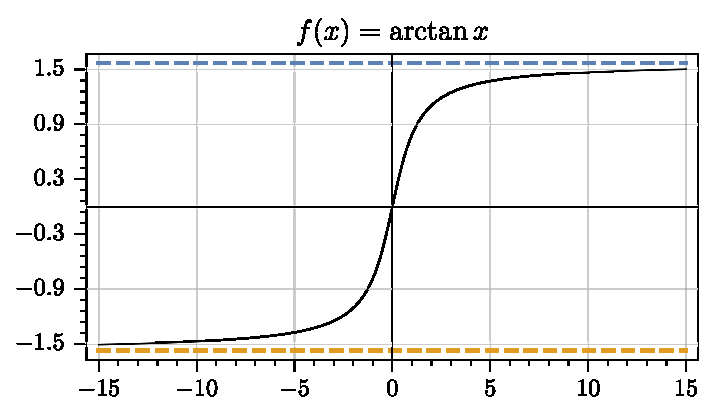
\includegraphics[width=0.7\textwidth]{1.eps}
    \caption{$f(x)=\arctan{x}$的图像}
  \end{figure}
  
\begin{definition}{无穷小}{wqx}
若 $ \lim\limits_{x \to a} \alpha(x)=0$,则称$ \alpha(x)$当$x \to a$时为无穷小。
\end{definition}

\begin{note}
\begin{enumerate}
  \item 0是无穷小,但无穷小不一定为0;
  \item $\alpha(x)\neq 0$,$\alpha(x)$是否为无穷小与$ x $的\CJKunderdot{趋向}有关;如,$\alpha=3(x-1)^2$,而$\lim\limits_{x \to 1}\alpha=0 $,则$3(x-1)^2$当$x \to 1$时是无穷小。
  \item 设$\alpha \to 0,\beta \to 0$,有如下三种情形:
  
  (a) $\lim \displaystyle\frac{\beta}{\alpha}=0$,称$ \beta $为$ \alpha $的高阶无穷小,记作$\beta=o(\alpha)$;
  
  (b) $\lim \displaystyle\frac{\beta}{\alpha}=k(\neq \infty,0)$,称$ \beta $为$ \alpha $的同阶无穷小,记作$\beta=O(\alpha)$(特例:$\lim \displaystyle\frac{\beta}{\alpha}$=1,则称$ \beta $与$ \alpha $为等价无穷小,记作$\beta \sim \alpha$)。
\end{enumerate}
\end{note}


\section{极限的性质}
下面我们开始介绍极限的有关性质,并给出相关的证明。主要有:唯一性、保号性(重点)两个性质。
\begin{enumerate}
    \item 唯一性
    \begin{property}
        极限存在必唯一。
    \end{property}
    
    \begin{proof}
    设$\lim\limits_{x \to a}f(x)=A $
    又$ \lim\limits_{x \to a}f(x)=B $,并不妨设$A>B$。我们采用反证法来完成相关的证明。
    
    取$ \varepsilon=\displaystyle\frac{A-B}{2}>0 $。因为$\lim\limits_{x \to a}f(x)=A $,所以存在$\delta_1>0 $,当 $0<\vert x-a\vert <\delta_1 $时,有$\vert{f(x)-A}\vert<\displaystyle\frac{A-B}{2}$,也即$\displaystyle\frac{A+B}{2}<f(x)<\frac{3A-B}{2}(*)$; 
    
    
    同理,由第二个极限可以得出$\displaystyle\frac{3B-A}{2}<f(x)<\displaystyle\frac{A+B}{2}(**)$。从而,若我们取$\delta=\min{(\delta_1,\delta_2)}$,当
    $ 0<\vert x-a\vert <\delta $时,就有$(*)$与$(**)$同时成立。但$f(x)>\displaystyle\frac{A+B}{2}$与$f(x)<\displaystyle\frac{A+B}{2}$显然不可能同时成立,矛盾,从而假设不成立。
    
    同理,我们可以得到$A<B$也不成立。故$A=B$。
    \end{proof}
    
    \item \FiveStar 保号性
    \begin{property}
        设$\lim\limits_{x \to a}f(x)=A>(<)0$,则存在$ \delta>0 $,当$ 0<\vert x-a\vert <\delta $时,有$f(x)>(<)0$。
    \end{property}
    \begin{proof}
        设$A>0$。取$\varepsilon=\displaystyle\frac{1}{2}A>0$。因为$\lim\limits_{x \to a}f(x)=A$,故存在$ \delta>0 $,当$ 0<\vert x-a\vert <\delta $时,有 $\vert{f(x)-A}\vert<\varepsilon=\displaystyle\frac{A}{2}$。展开可得$\displaystyle\frac{A}{2}<f(x)<\displaystyle\frac{3}{2}A$。从而$f(x)>0$。
    \end{proof}
    \begin{example}
        \item
    \end{example}
\end{enumerate}


\end{document}
